% Original book diagram: fig:sigma_points
% Book source: sections/Part_II/ukf.tex
% Original diagram authorship retained. Visual design: Ziad Mosalam.
\documentclass[11pt,border=8pt]{standalone}
\usepackage{amsmath,amssymb,graphicx,tikz}
\usetikzlibrary{arrows.meta,automata,positioning,calc,shapes.geometric,fit,backgrounds,patterns}
\newcommand{\vect}[1]{\mathbf{#1}}
\newcommand{\mat}[1]{\mathbf{#1}}
\newcommand{\Normal}{\mathcal{N}}
\newcommand{\prob}{p}
\newcommand{\E}{\mathbb{E}}
\newcommand{\Var}{\mathrm{Var}}
\newcommand{\Cov}{\mathrm{Cov}}
\newcommand{\CovP}{\mathbf{P}}
\newcommand{\Prob}{\mathbb{P}}
\setlength{\textwidth}{6.5in}
% Shared visual vocabulary for the book's original diagrams.
% Figures opt in explicitly, so unrelated text and existing additions are unchanged.
\definecolor{BookBlue}{HTML}{003262}
\definecolor{BookGold}{HTML}{B17A00}
\definecolor{BookTeal}{HTML}{247C86}
\definecolor{BookInk}{HTML}{30363B}
\definecolor{BookLight}{HTML}{E9EFF5}
\tikzset{
  book figure/.style={font=\small\rmfamily, color=BookBlue, text=BookInk,
    line width=0.8pt, >=Latex},
  book axis/.style={->, draw=BookInk, line width=0.6pt},
  book link/.style={->, draw=BookBlue, line width=0.8pt},
  book observation/.style={draw=BookGold, fill=BookGold!8},
  book state/.style={draw=BookBlue, fill=BookLight},
  book note/.style={font=\footnotesize\rmfamily, text=BookInk}
}

\begin{document}
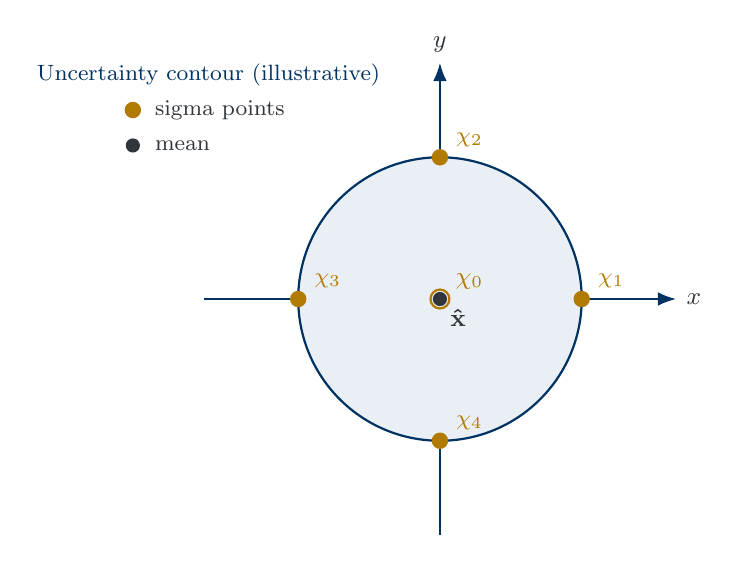
\begin{tikzpicture}[font=\small, text=BookInk, draw=BookBlue, line width=0.8pt, >=Latex, scale=1.5,>=Latex]
  % Axes
  \draw[->] (-2,0) -- (2,0) node[right] {$x$};
  \draw[->] (0,-2) -- (0,2) node[above] {$y$};

  % Uncertainty "ellipse" (here shown as circle for simplicity)
  \fill[BookLight] (0,0) circle (1.2);
  \draw[BookBlue, line width=0.8pt] (0,0) circle (1.2);

  % Mean (black dot)
  \fill[BookInk] (0,0) circle (0.06);
  \node[below right] at (0,0) {$\vect{\hat{x}}$};

  % Sigma points (red) + labels
  \foreach \x/\y/\lab in {1.2/0/{\vect{\chi}_1}, -1.2/0/{\vect{\chi}_3}, 0/1.2/{\vect{\chi}_2}, 0/-1.2/{\vect{\chi}_4}} {
    \filldraw[BookGold] (\x,\y) circle (0.06);
    \node[BookGold] at (\x+0.25,\y+0.15) {\footnotesize $\lab$};
  }
    \draw[BookGold] (0,0) circle (0.08);
    \node[BookGold] at (0.25,0.15) {$\vect{\chi}_0$};

  % A small legend / callouts
  \filldraw[BookGold] (-2.6,1.6) circle (0.06);
  \node[anchor=west] at (-2.5,1.6) {\footnotesize sigma points};
  \fill[BookInk] (-2.6,1.3) circle (0.06);
  \node[anchor=west] at (-2.5,1.3) {\footnotesize mean};

  \node[BookBlue,anchor=west] at (-3.5,1.9) {\footnotesize Uncertainty contour (illustrative)};
\end{tikzpicture}
\end{document}
